%!TEX root = ../report.tex

\begin{document}
  \chapter{Experimental Setup}

  Having applied the theoretical knowledge derived in Section 3 to the ROPOD case
  study in Section 4 we have begun to narrow down the options for spatio-temporal
  world modeling in this particular case. However, a theoretical comparison will
  only suffice for so long. Given the focus ROPOD places on real world
  environments it is critical that some operational tests be preformed before
  method selection. Not only will these experiments serve as a guide for ROPOD,
  but they will also act as a template for the comparison of future
  spatio-temporal world modeling techniques.


  \section{ Environmental Representation}

  Given the complexity and size of the target environment for ROPOD, a large
  hospital, it is necessary to pair down features of the building until only
  the core components remain. The three dynamic environmental components being
  target are doors, path planning with carts that are often strewn about the
  hallways and surrounding rooms, and elevators. Therefore, a model
  environment has been designed for the simulations to be run on that contains
  these three key components.  The model environment that has been designed
  takes heavy influence from the actual environment but some notable have been
  made. The model has a decreased area to allow for faster model training and
  path planning. Additionally, extraneous rooms and hallways have been
  removed. A comparison between the actual hospital and the designed model can
  be seen below.

  TODO add picture


  \section{ Common Assumptions }
  In order to insure only the desired component is being tested at any given
  time a set of assumptions are made.

  \begin{itemize}

    \item All robot components are working correctly (no internal faults)

    \item Other than the object under test (e.g. doors), all other objects in the
          environment are static

    \item All information other than the objects under test are perfectly known

    \item Observations made/provided by the training data are assumed to be
          ground-truth

  \end{itemize}


  \section{ Commonalities in Approach }
  Although different components will be under test, each experiment will be run
  in a similar manor.

  The experimental setup is as follows:

  \begin{itemize}

    \item Training data consisting of observations made every 15 minutes over
          a simulated month will be provided to the models

    \item All data generation will be done using the same program and the
          specifics of how the data is generated will be discussed further
          below in the relevant experiment section

    \item Using the same generation procedure, a new month will be generated

    \item The models will be trained using the original month and then tested
          against both the original month and the new test month

    \item In the case of the doors and elevator, only the objects themselves
          will be modeled and the comparison will only be how well the generated
          models can predict the ground thruth

    \item In the case of the more advanced hallway scenario, predictions about
          objects in the environment will be used to plan a path and this path
          will be compared with paths planned using the ground truth

    \item All of these paths will then be compared using the criteria described
          below.

    \item All experiments will be done on the same hardware
      \begin{itemize}
        \item ASUS UX330UAK Laptop
        \item i5-7200k 2.5GHz
        \item 8GB DDR3
        \item Arch Linux 4.19.4
      \end{itemize}

  \end{itemize}

  \section{ Data Generation }

  Data generation is done using a combination of built in Python libraries and
  the NumPy library. Each object is broken down into a series of days which is
  then further broken down into a series of behaviors. Each behavior
  represents the likelihood of an object being in a given state between two
  times.  Furthermore, each behavior has a starting state and an ending state,
  which if different, are swept through linearly. E.g. if a behavior is
  modeling a binary state of a door that starts at 100\% open and then becomes
  100\% closed an hour later at the half hour mark the door would have the
  door being at a 50\% likelihood of being open. Additionally, it is possible
  to specify the amount of Gaussian noise that is added on top of the
  behavior where the nominal state is used as mu and the sigma is used to
  specify the magnitude of the noise. Months of data are thus generated by
  walking through these behaviors in 15 minute increments for each day in the
  month where each month is assumed to have exactly 31 days.

  For example, if a door was open from noon until midnight every day, and then closed from
  midnight until noon there would be two behaviors one from midnight until
  noon and one from noon until right before midnight. In this case, the
  starting and ending values of each behavior would be the same and no noise
  would be introduced. This would create a sharp, well defined change at
  exactly noon and midnight every day. Further details and specifics about data
  generation will be discussed in their respective sections.

  \section{ Model Parameters }
  TODO: add section to talk about how model params where chosen


  \section{ Comparison Criteria }
  In order to evaluate the intricacies of the selected models a wide variety
  of data points have been selected for comparison. A focus has been placed on
  collecting data relevant to accuracy and scale-ability of the modeling
  technique given the eventual scope of the ROPOD project.

  \begin{itemize}

    \item Accuracy to Ground Truth

    \item Accuracy to Historical Recreations

    \item Planning Run-time

    \item Planning Memory Consumption

  \end{itemize}

  \section{ Doored Areas}

  \subsection{ Experimental Motivation }

  As is the case in many places of employment many areas of a building may not
  be accessible to the public, and by extension the robots, outside of work
  hours.  This could come in the form of a given hallway between two areas being
  locked after 17:00 as the day works go home. In another case, it could be as
  simple as someone preferring to having a door shut to a hallway during a loud
  or chaotic time of the day. \\

  Regardless of the reason, it is certain that the states of doors are often
  both dynamic exhibiting both periodic and long term changes. In the ideal case, a robot, much like humans,
  would learn when certain doors are closed and be able to plan accordingly.
  Making an accurate prediction can save time, but making an inaccurate
  predication can also be costly. An in accurate prediction would force a robot
  to not only backtrack, but also recalculate that path required to get to a
  target. Additionally, it may not be possible to make deliveries at all times.
  In the worse case, a robot may even manage to get itself locked in an
  environment unable to return back to it's base and eventually run out of power
  requiring human intervention. For these reasons and many more, the door
  experiment is an excellent example of the benefits of spatio-temporal world
  modeling. \\

  \subsection{ Experimental Details }

  In order to keep this test as straight forward as possible, only the door
  object itself has been modeled. The doors could belong to a room where a
  package must delivered or perhaps a hallway that could be used as a
  shortcut. Each model will be directly, or indirectly be tasked with
  predicting the state of this door. Figure 5.1 displays an example of three
  doors in ward 24 of the hospital that may display the dynamic behavior
  previously mentioned. \\

  When evaluating the predictions made by the models a simple 50\% confidence
  value will be used. That is to say, if a model predicts that the door will
  be 50\% or more likely to be open will result in the robot attempting to
  deliver the package. \\

  \begin{figure}[!htb]
    \centering
    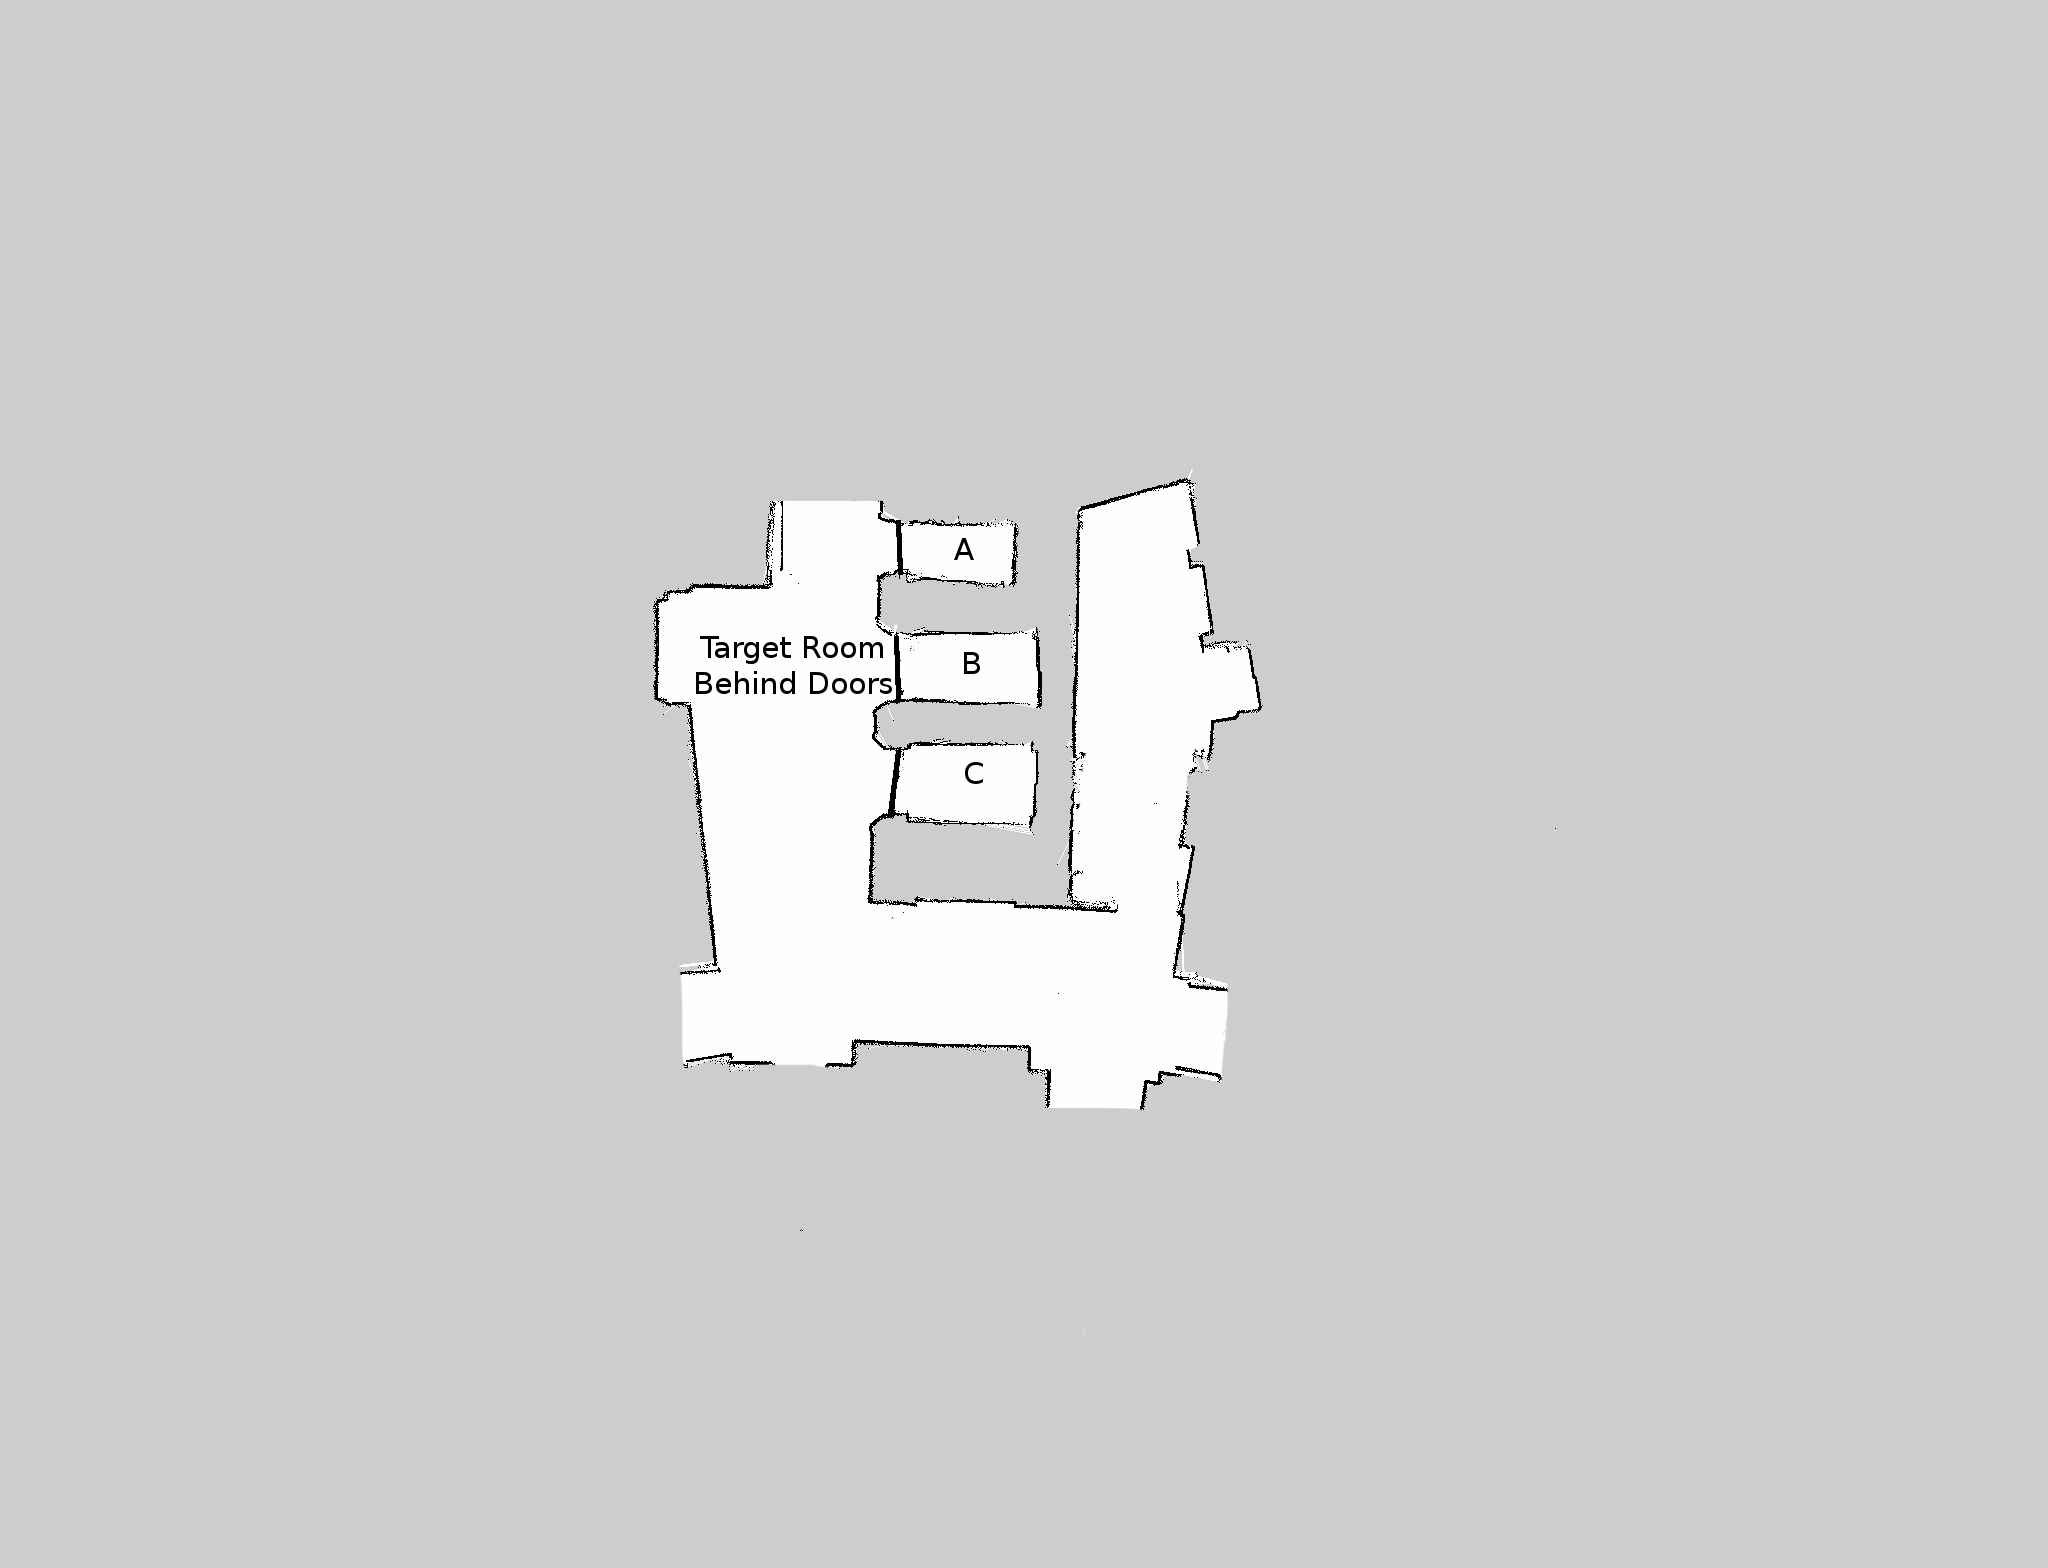
\includegraphics[width=\linewidth]{images/ward_24_door.png}
    \caption{Multiple rooms behind doors in ward 24.}
    \label{figure:ward_24_door}
  \end{figure}

  It is clear that this 50\% cutoff does not take into account the penalties
  of making a wrong prediction, but this particular experiment was designed to
  investigate the accuracy of the prediction. The hallway experiment discussed
  below will delve a little deeper into the ramifications of inaccurate
  predictions. That being said, how the information of the prediction is
  handled afterwards is undoubtedly valuable, but is outside the scope of this
  current research.

  \subsection{ Data Generation }

  As mentioned above, both the training and the test data for all models was
  generated using the same program.

  The specifics for each door are as follows.

  \subsection{ Door A }

  Door A is models a door that is highly influenced by the daily schedule of a
  9:00 to 17:00 job and has a high amount of periodic behavior with a small
  amount of noise.  There are 5 behaviors which model a standard work day. The
  time from midnight until work starts at 9 has the door in a normally closed
  state.  From 9:00 until 12:00 the door is likely open. 12:00 until 13:00 is
  considered lunch time and thus the door is likely closed. Work resumes at
  13:00 until 17:00 and thus likely open. From 17:00 until midnight
  the door remains in a likely closed state. Finally, the door is always
  closed on weekends with a 100\% probability and no noise. \\

  When the door is in a likely open state it has 70\% chance of being open.
  Likewise, when in a likely closed state it has a 70\% chance of being closed.
  Finally, when noise is introduced during the weekday it uses a standard deviation
  of 0.1 where mu is either 0.3 or 0.7 and 0.5 is the cutoff for being open or
  closed. \\

  \begin{figure}[!htb]
    \centering
    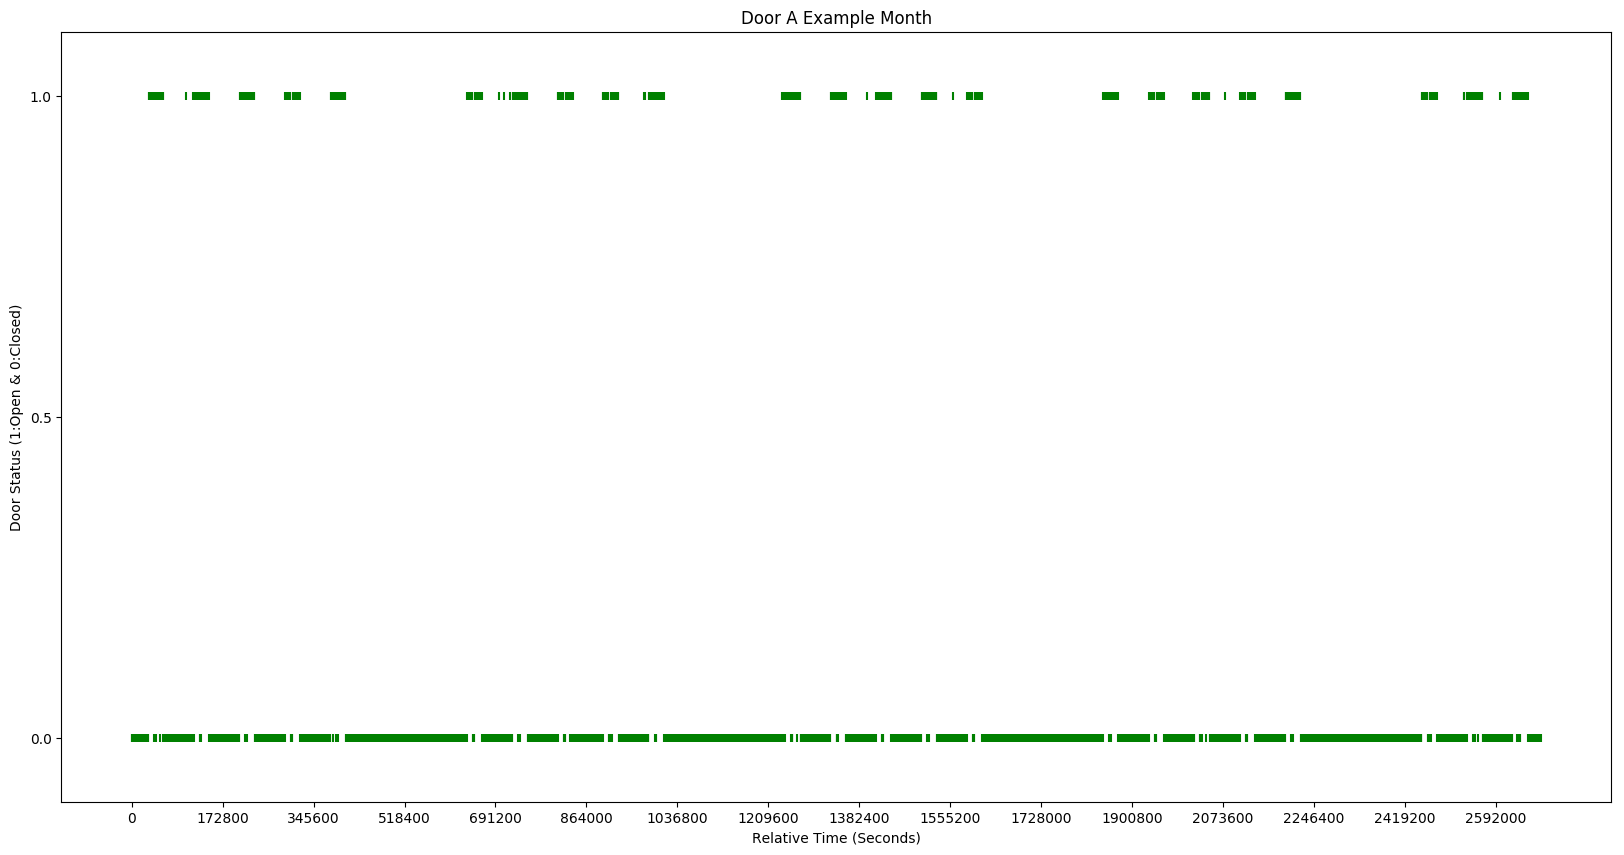
\includegraphics[width=\linewidth]{images/Door_A_Example_Month.png}
    \caption{The training data for Month A}
    \label{figure:Door A Training Month}
  \end{figure}

  \subsection{ Door B }

  Door B, in a similar manor to door A, also tries to encapsulate the periodic
  behaviors of a work day but with a little more noise. Door B is always open
  from midnight until the start of the work day at 9:00. During the work day
  the door is a constant state of flux, being open and shut at random. This is
  modeled using a mu of 0.5 and a standard deviation of 0.1. This ends when
  the work day is over at 17:00 and the door goes back to remaining open until
  the next work day starts. To add additional periodic complexity, such as a
  weekly meeting or delivery, every third weekday the door will be closed the
  entire day. This trend is continued across month boundaries. This means if
  the doors was closed on the day before the last day of the first month it
  will again be closed on the second day of the next month. Finally, on
  weekends the door will always be open with 100\% certainty and no noise. \\

  \begin{figure}[!htb]
    \centering
    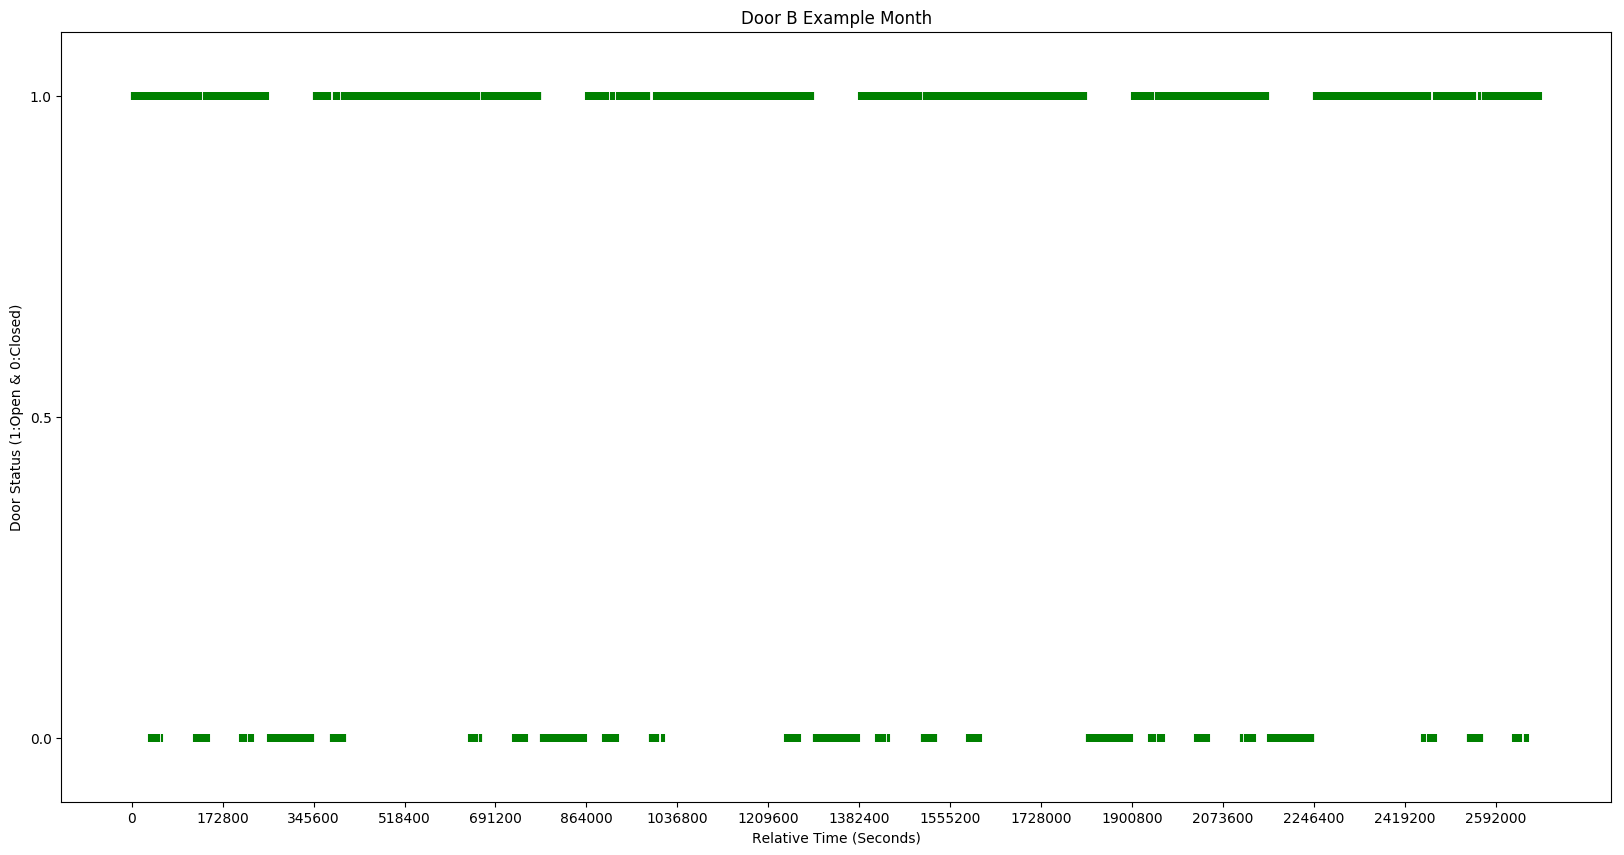
\includegraphics[width=\linewidth]{images/Door_B_Example_Month.png}
    \caption{The training data for Month B}
    \label{figure:Door B Training Month}
  \end{figure}

  \subsection{ Door C }

  Door C does not attempt to model any periodic behavior but instead test
  long-term change in an environment. A simple illustration of the long-term
  non-periodic change could be that of construction. The door has always been
  open in the past but it leads to a wing of the building that is now either
  being remodeled or has been removed. In the test data, this behavior is
  achieved by having the door be open for the first three weeks and then being
  closed for the rest of the training month and through the test month. In
  this model no noise was introduced. \\

  \begin{figure}[!htb]
    \centering
    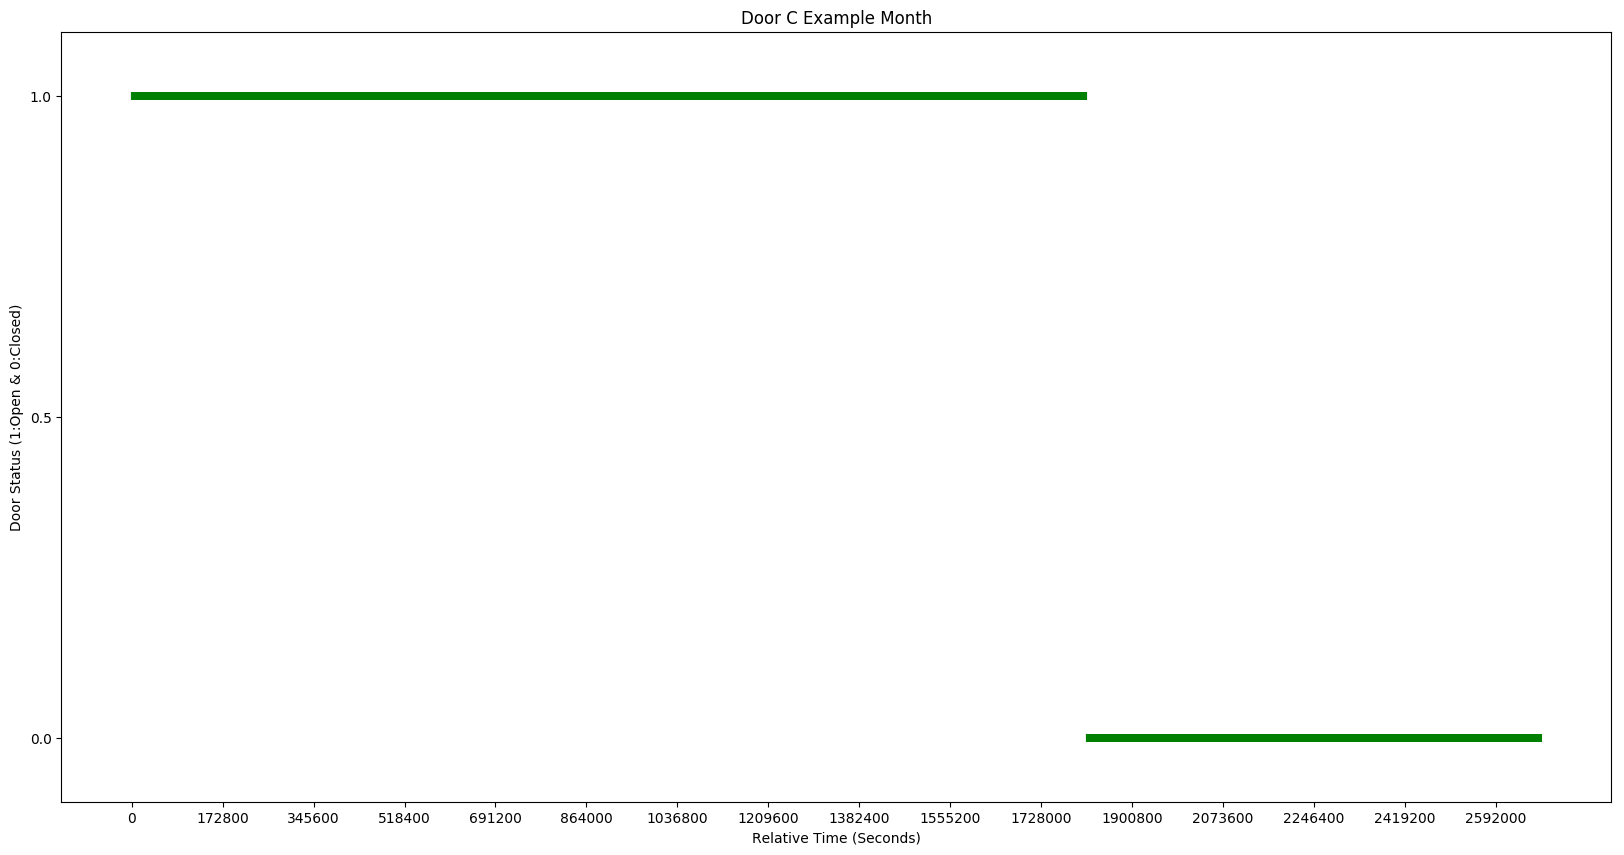
\includegraphics[width=\linewidth]{images/Door_C_Example_Month.png}
    \caption{The training data for Month C}
    \label{figure:Door C Training Month}
  \end{figure}

  \section{ Congested Hallways }

  \subsection{ Experimental Motivation }



  \subsection{ Experimental Details }

  Figure 5.3 displays the starting and goal point of the
  desired path. In order to keep this test as straight forward as possible, only
  one door has been included. The door belongs to a hallway that acts like a
  shortcut between the two other hallways. Each model will be directly, or
  indirectly tasked with predicting the state of this door. A simple 50\%
  confidence value will be used. That is to say, if a model predicts that the
  door will be 50\% or more likely to be open that path will be taken. \\


  \begin{figure}[!htb]
    \centering
    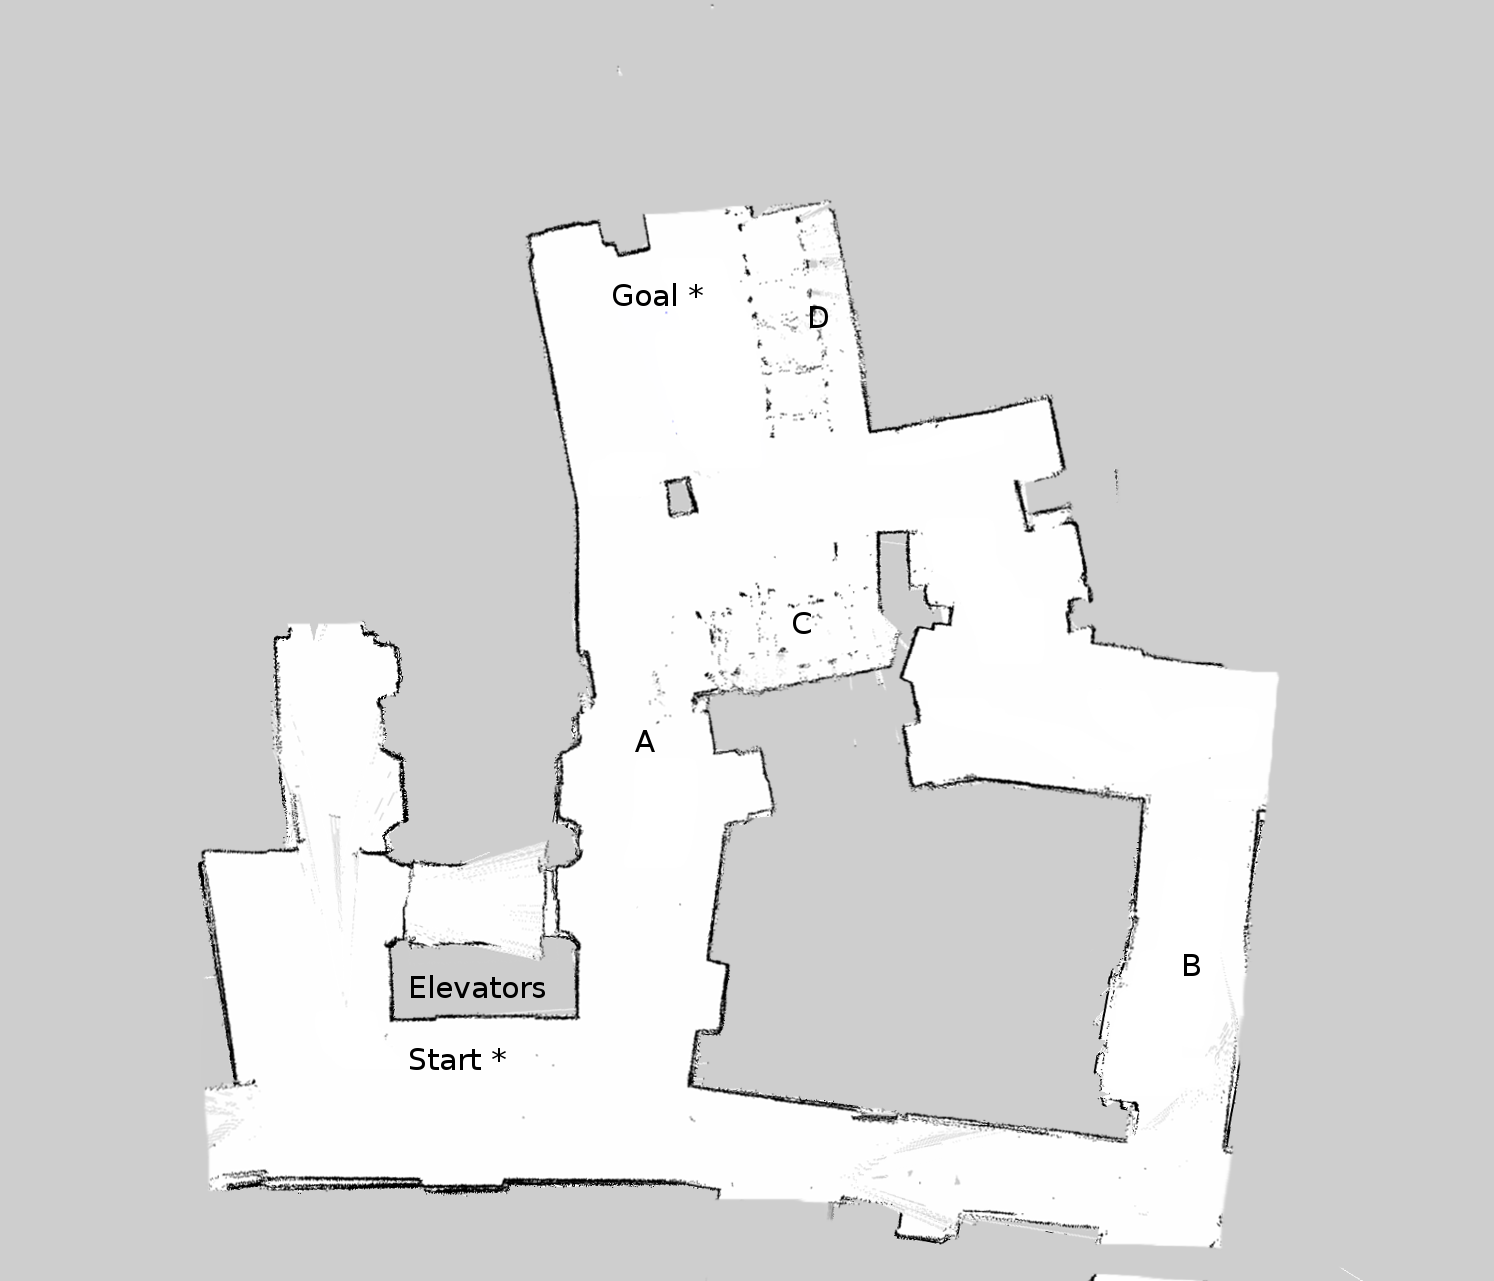
\includegraphics[width=\linewidth]{images/basement_congestion.png}
    \caption{The path from the elevator to the storage area is often congested. }
    \label{figure:basement_congestion}
  \end{figure}

\end{document}
